\chapter{Resultados}

El editor resultante es un editor ligero y fácil de usar que puede insertarse en una página con apenas dos líneas de código (ver apéndice Integración en la plataforma SWAD). Se han realizado una serie de pruebas sobre el editor y aunque aún no se ha incorporado totalmente en la plataforma se han obtenido muy buenos resultados.

Durante el desarrollo del editor se han ido realizando pruebas en la página de test de la figura ~\ref{fig:result_testpage0}.

\begin{figure}[h!]
  \centering
      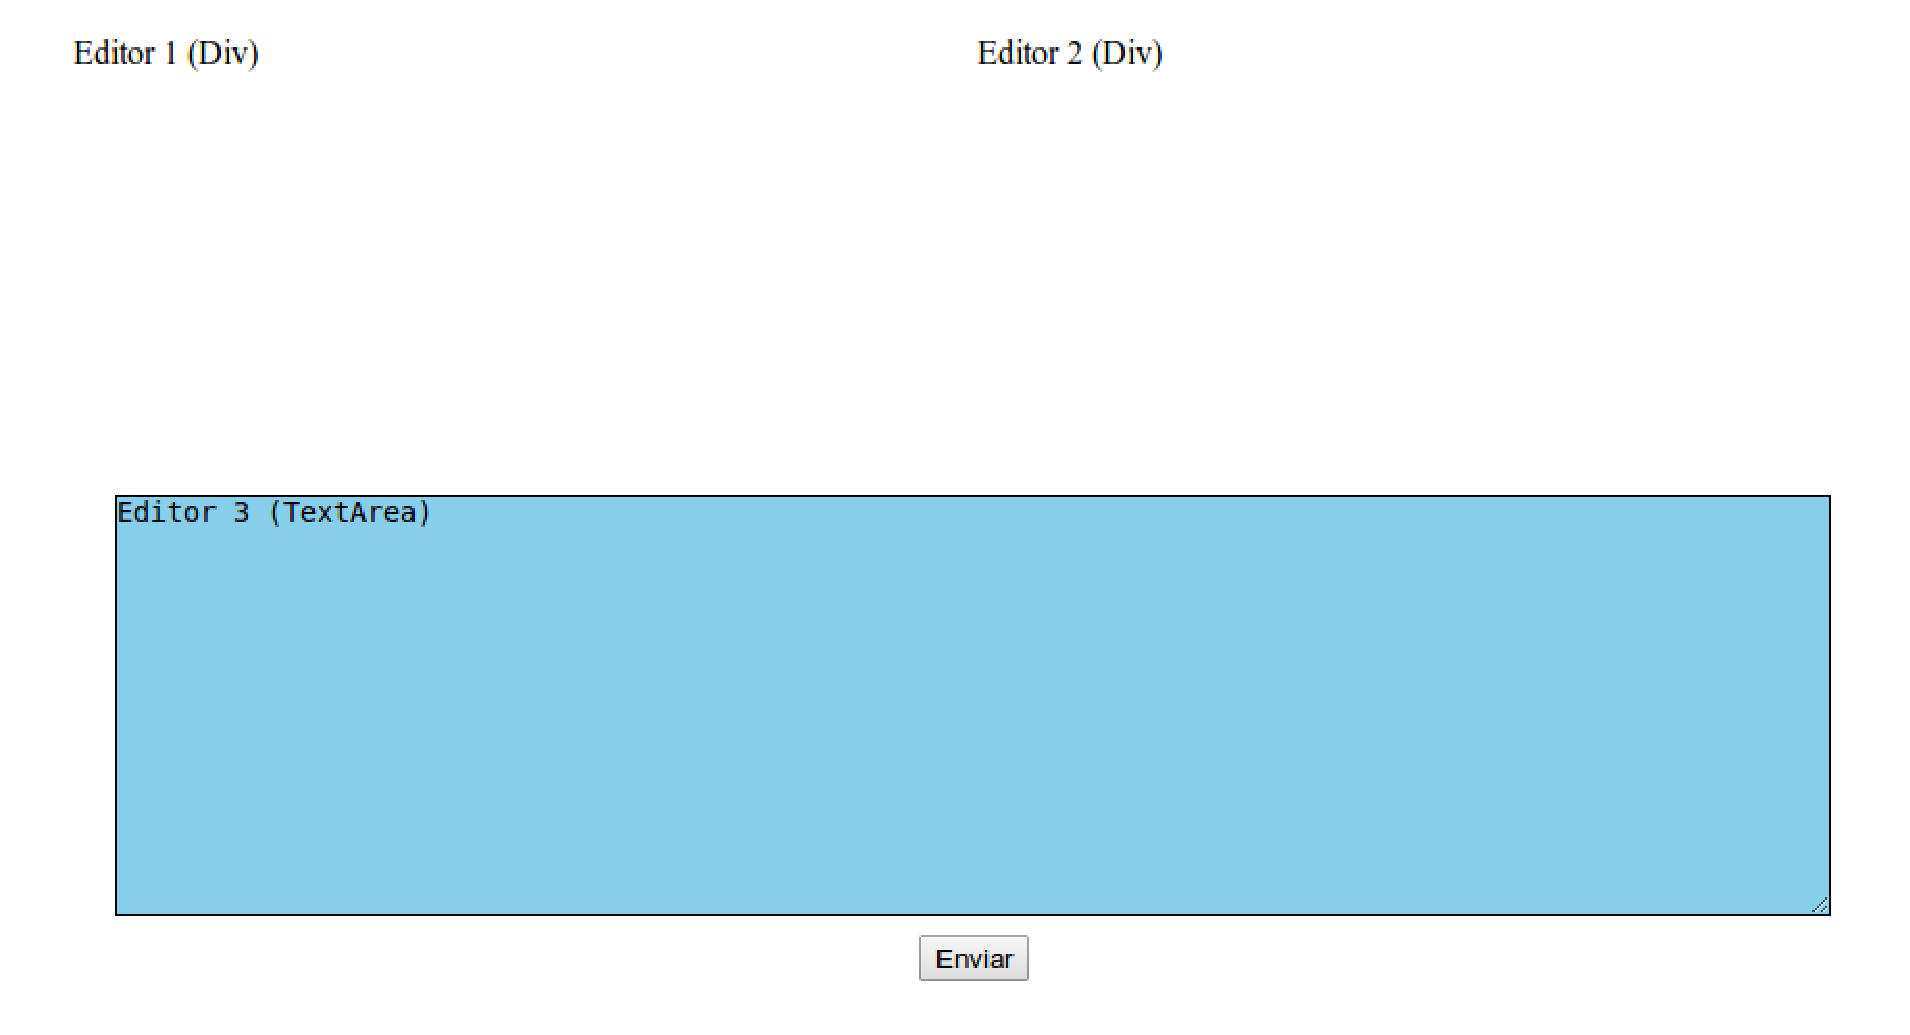
\includegraphics[width=7in]{fig/result_testpage0}
  \caption{Página de pruebas sin SWADE}
  \label{fig:result_testpage0}

\end{figure}


Esta página posee dos elementos div y un textarea, identificados por el atributo HTML clase ``swade''. Insertando en la cabecera de la página las líneas de código siguientes:
\begin{verbatim}
<script src="../swade.js" type="text/javascript"></script>
<script>
  SwadeManager.setOnDOMLoaded(function(){
  SwadeManager.setSwadeByClassName("swade");});
</script>
\end{verbatim}

Nuestro editor hará el resto del trabajo, transformando los tres elementos citados en editores SWADE. Ver figura ~\ref{fig:result_testpage1}.

\begin{figure}[h!]
  \centering
      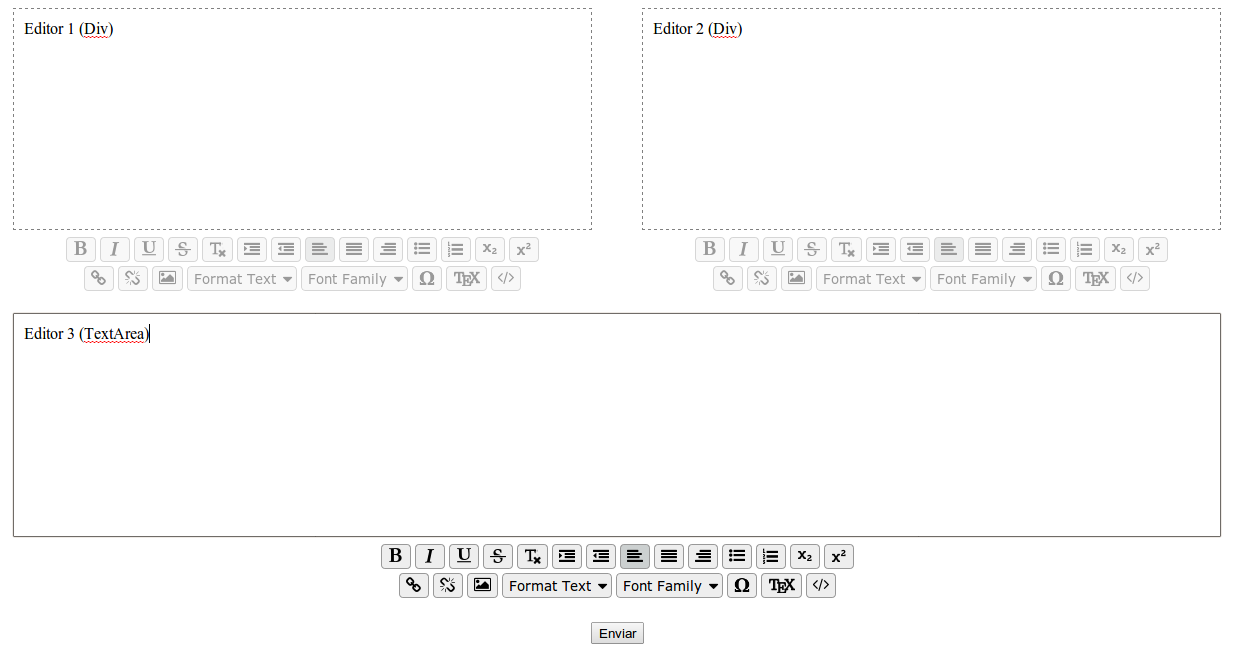
\includegraphics[width=7in]{fig/result_testpage1}
  \caption{Página de pruebas con SWADE}
  \label{fig:result_testpage1}

\end{figure}


Esta página contiene también un formulario cuyos únicos elementos son el textarea inferior y el botón de submit, responsable de enviar el contenido del textarea. Nuestro editor se ocupará de interceptar el evento de pulsación del botón para asignar el contenido del editor al textarea antes de ser enviado. De esta forma se enviará el código HTML que contiene el editor.

\begin{figure}[h!]
  \centering
      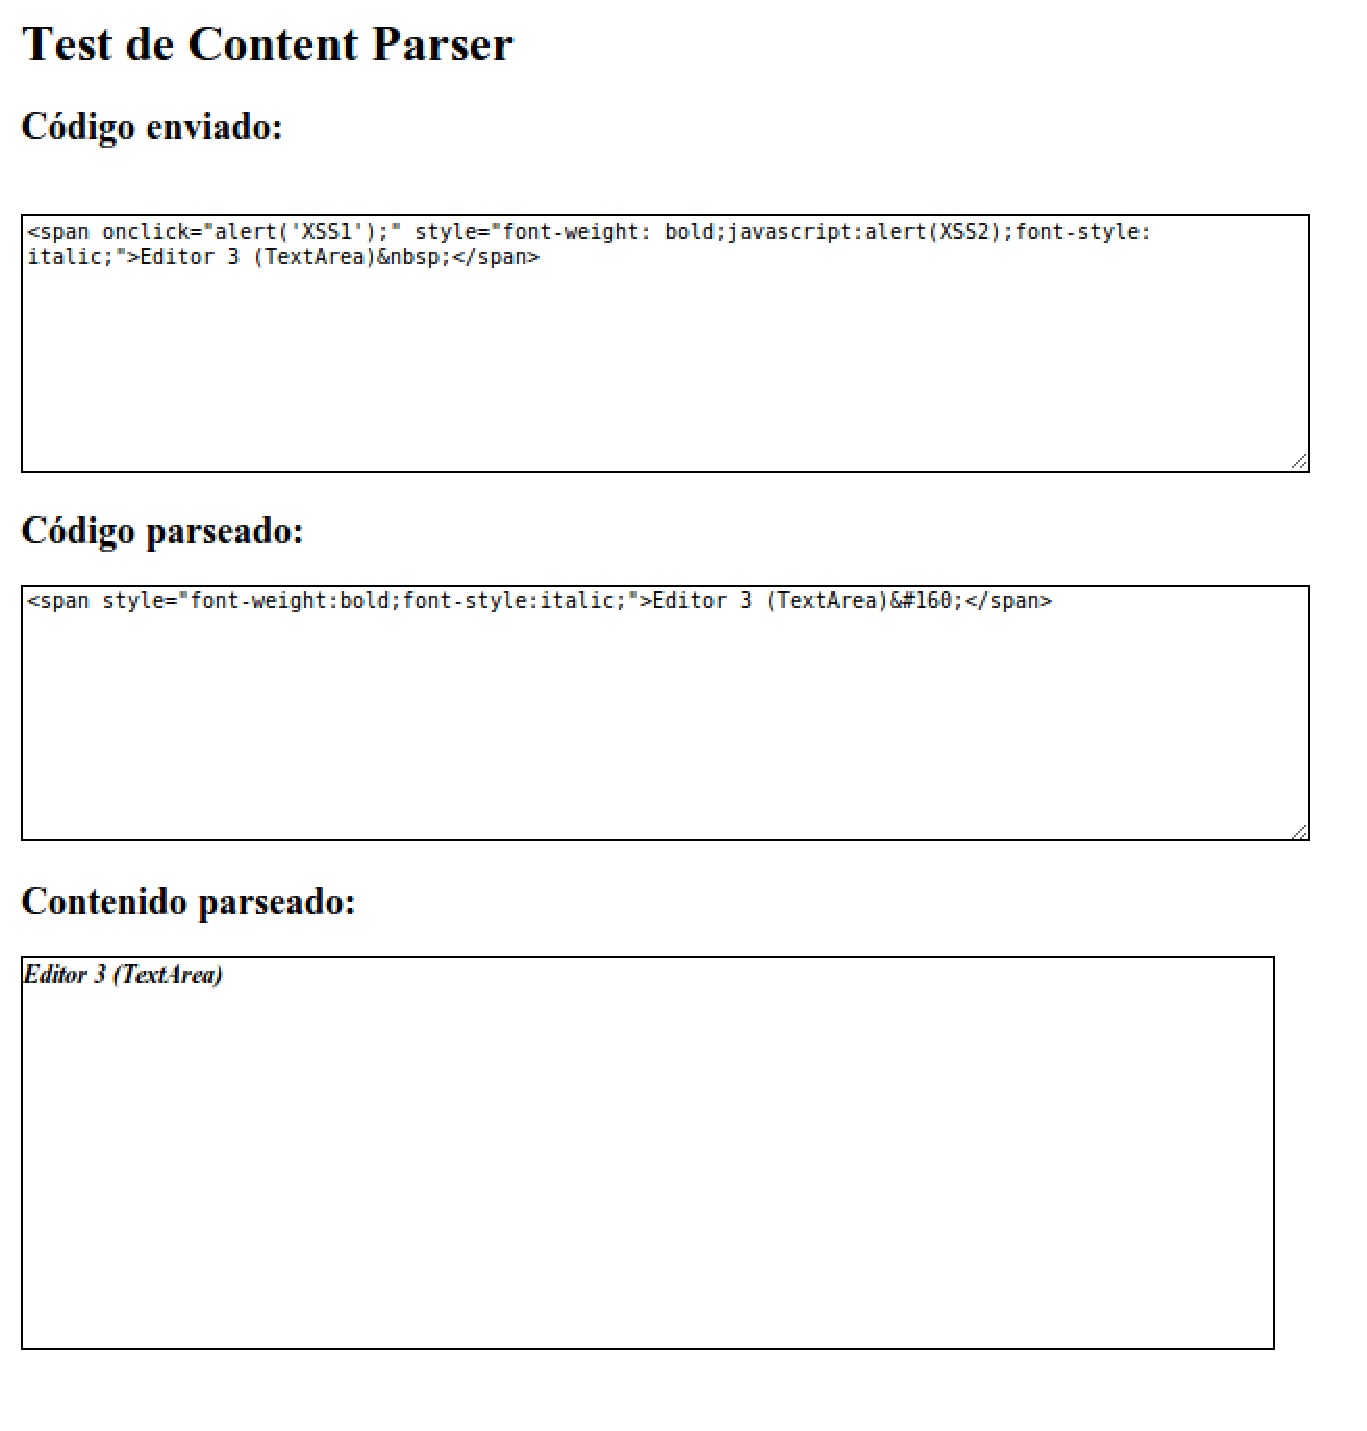
\includegraphics[width=5in]{fig/result_testpage2}
  \caption{Páginas de pruebas de limpieza HTML}
  \label{fig:result_testpage2}
\end{figure}

Para probar el filtrado HTML se ha usado la página de las figura ~\ref{fig:result_testpage2}. Esta página es un script php que recoge el valor enviado por el formulario y muestra su valor filtrado y sin filtrar, además de renderizar el HTML filtrado.


En las figuras ~\ref{fig:result_testpage3} y ~\ref{fig:result_testpage4} podemos ver el envío de símbolos y fórmulas.

\begin{figure}[h!]
  \centering
      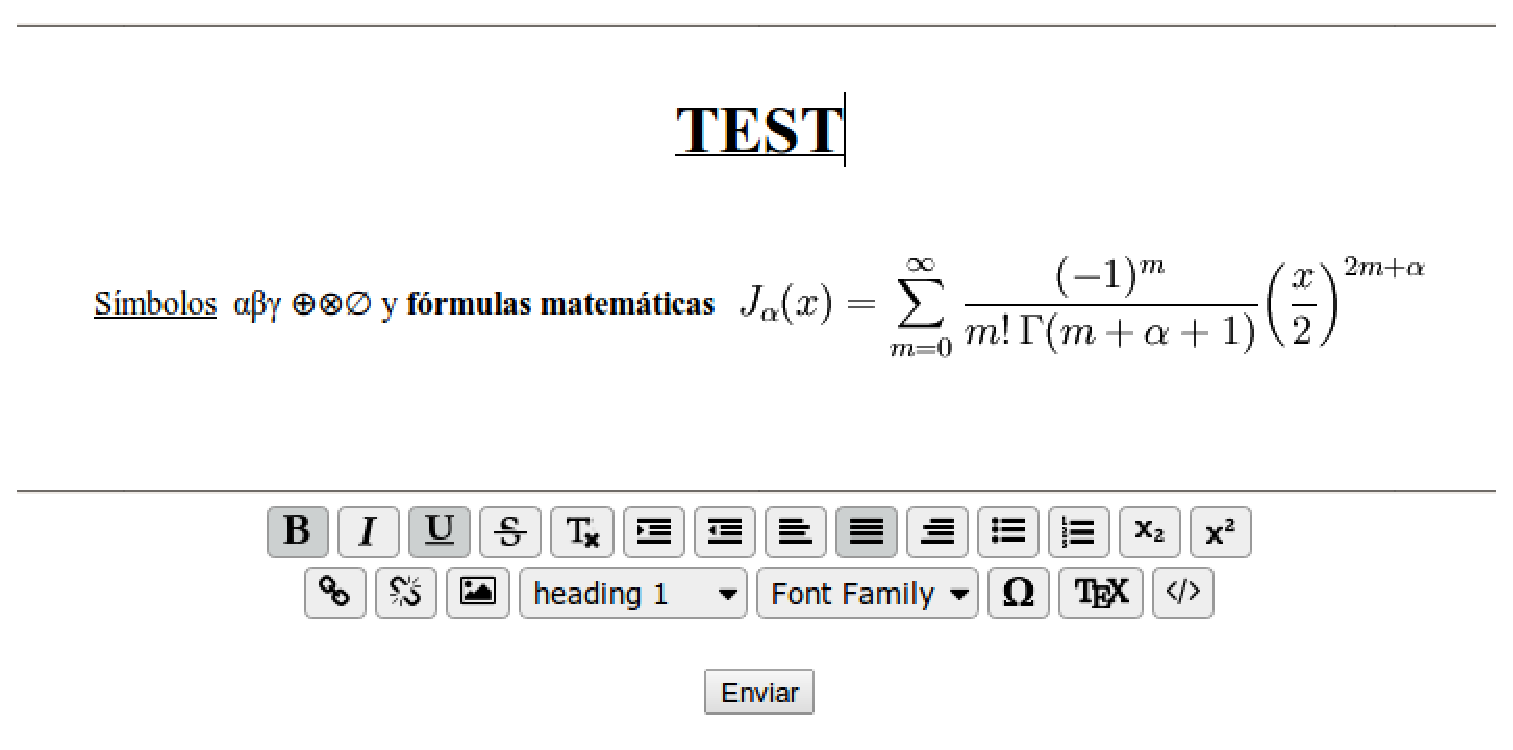
\includegraphics[width=5in]{fig/result_testpage3}
  \caption{Envío en un formulario de símbolos y fórmulas.}
  \label{fig:result_testpage3}

\end{figure}


\begin{figure}[h!]
  \centering
      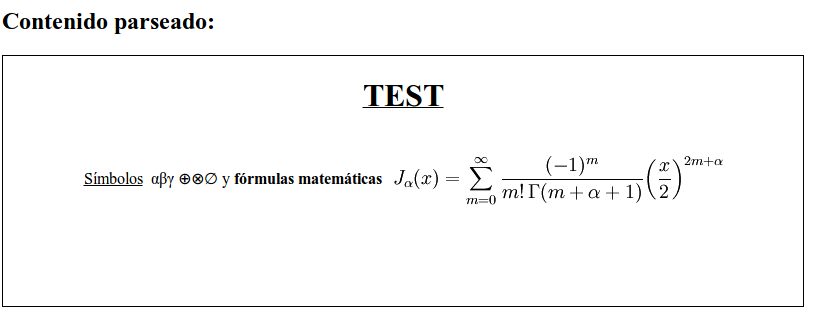
\includegraphics[width=5in]{fig/result_testpage4}
  \caption{Limpieza del HTML en el servidor y renderizado del contenido enviado en el formulario.}
  \label{fig:result_testpage4}

\end{figure}

Una vez testeada la funcionalidad del editor, hicimos algunas pruebas de integración en las secciones descritas en el capítulo de Análisis. 

En la figura ~\ref{fig:swade_test1} podemos ver el editor integrado en la sección de envío de mensajes y en las figuras ~\ref{fig:result_test1} y ~\ref{fig:result_test2} lo vemos en la sección de Test. 

\begin{figure}[h!]
  \centering
      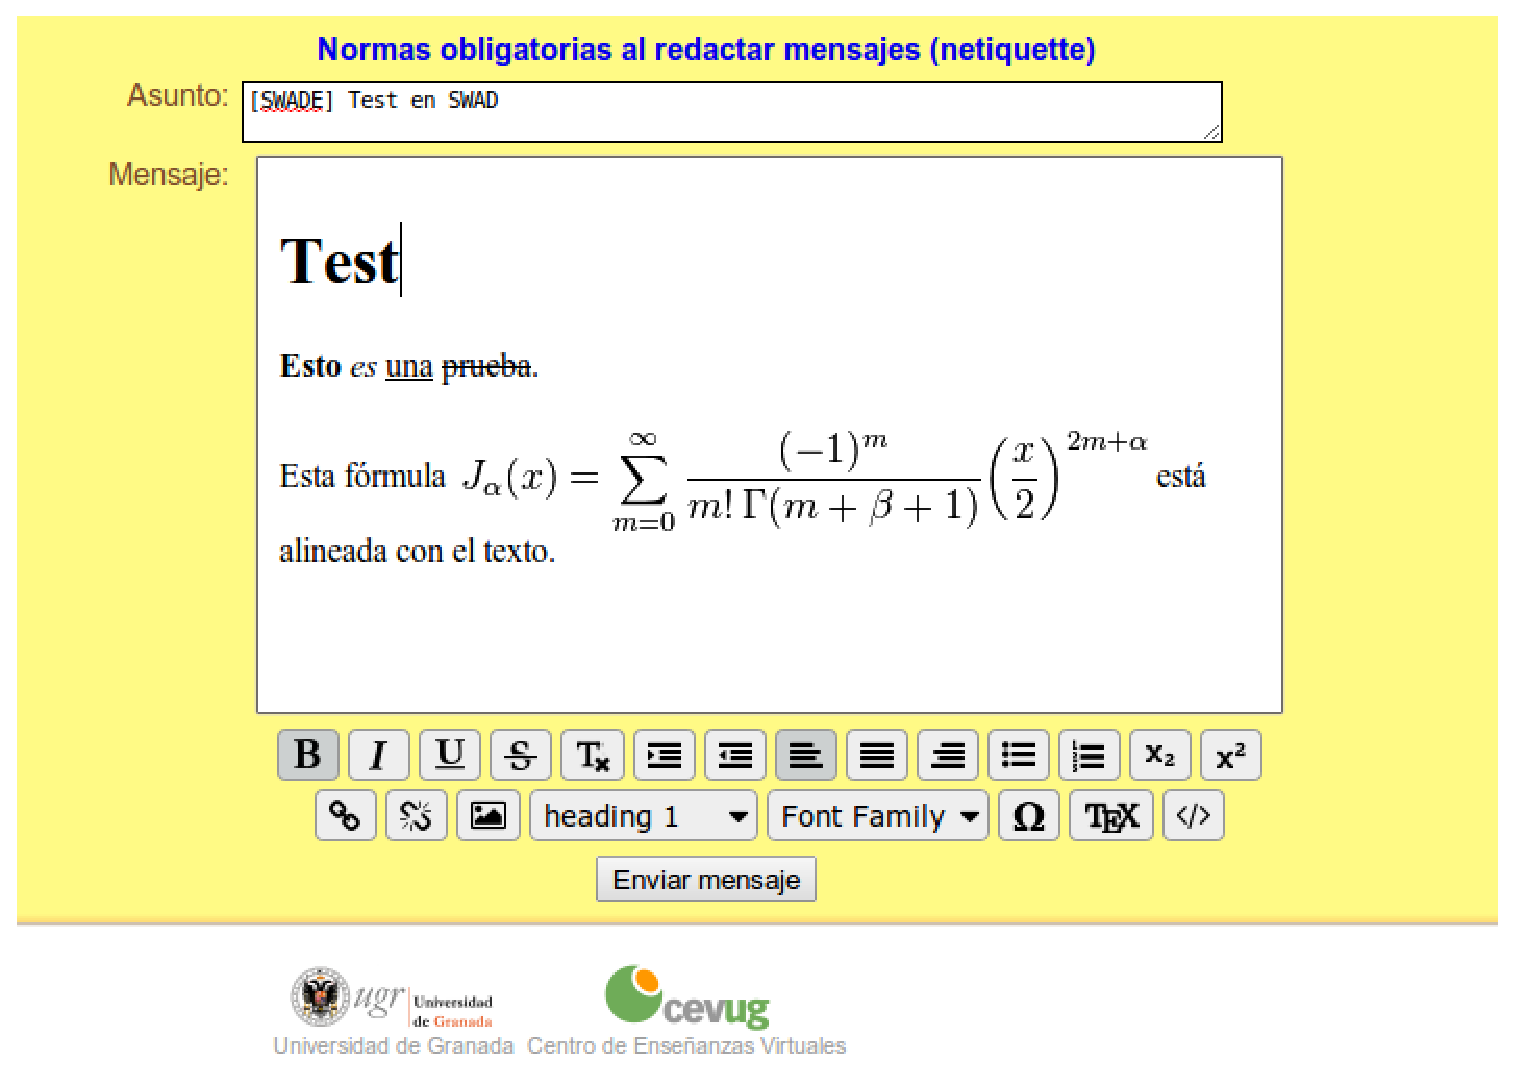
\includegraphics[width=5in]{fig/swade_test1}
  \caption{SWADE en mensajes}
  \label{fig:swade_test1}

\end{figure}


\begin{figure}[h!]
  \centering
      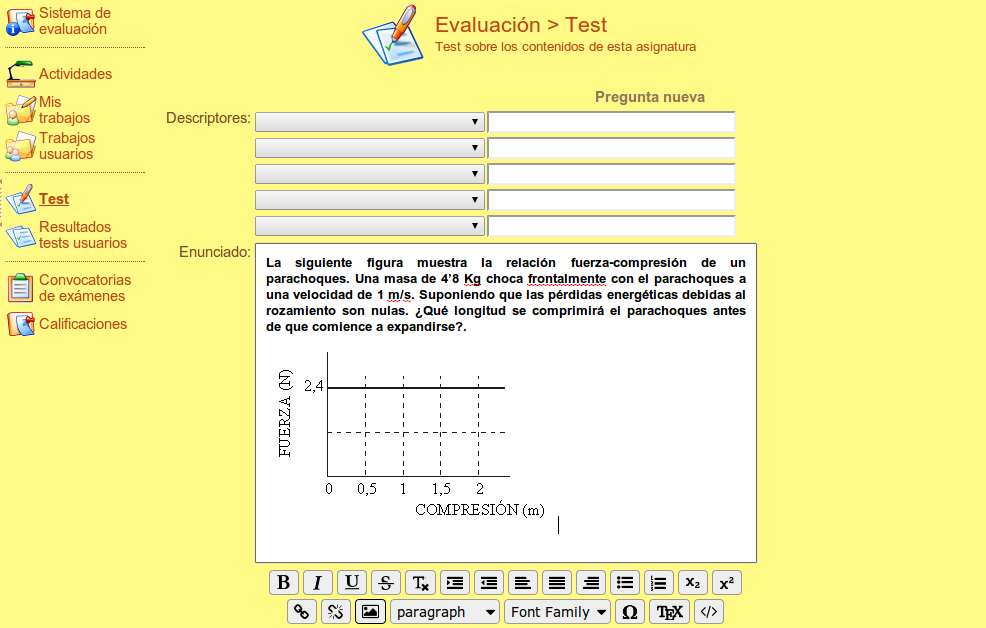
\includegraphics[width=5in]{fig/result_test1}
  \caption{SWADE en preguntas de Test}
  \label{fig:result_test1}

\end{figure}


\begin{figure}[h!]
  \centering
      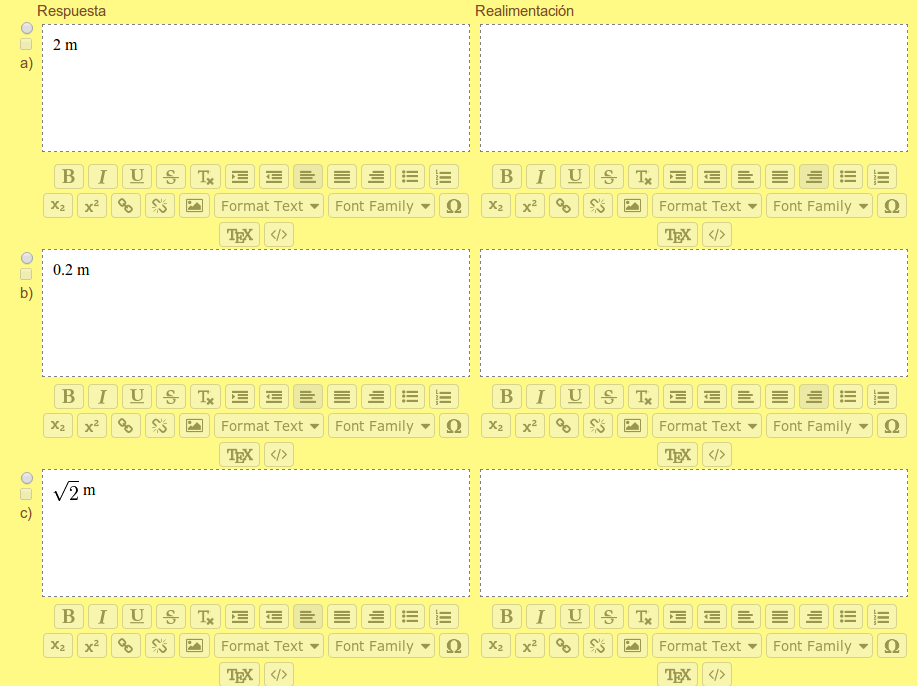
\includegraphics[width=5in]{fig/result_test2}
  \caption{SWADE en respuestas de Test}
  \label{fig:result_test2}

\end{figure}


